\nextpage
\section{Одна лексика, четыре реализации}
Учебный псевдокод допускает математическую запись \sourcega{0.2.4}{1/5}. Для опыта мы зафиксировали её байтовое представление. Идентификатор начинается с латинской буквы и продолжается буквами или цифрами. Число состоит из одной или нескольких десятичных цифр. Это два класса слов, задаваемых регулярными выражениями \cite[п.~1.2.1, слайды 1/3--2/3]{ga}. Ещё 11 видов отведены ключевым словам и 18~--- знакам и разделителям. Всего сканер различает 31 обычный вид лексемы.

В каждой позиции выбирается самое длинное подходящее слово. При равной длине ключевое слово имеет приоритет над идентификатором. Пробел, табуляция, возврат каретки и перевод строки пропускаются. Комментарий \code{//} продолжается до конца строки или входа. При ошибке в позиции $p$ сканер выдаёт интервал $[p,p+1)$, в конце текста длины $N$~--- признак конца файла (EOF, от английского \textnormal{end of file}) с интервалом $[N,N)$. Позиции нумеруются с нуля. В правую границу интервала байт уже не входит.

Для каждого вида лексемы нужны состояния, в которых прочитанное слово можно принять. В модели автомата-распознавателя это заключительные состояния \sourcega{2.2.1}{1/2}. Сканер дополнительно хранит вид принятого слова и его правую границу.

\begin{center}
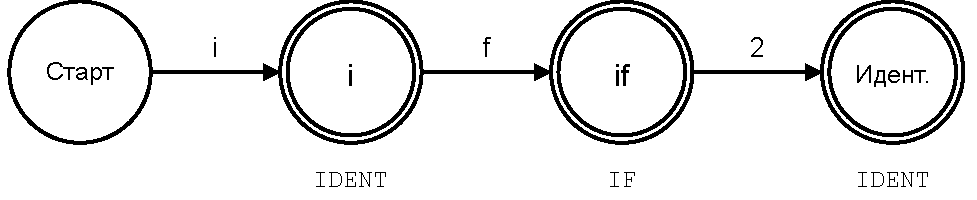
\includegraphics[width=.85\linewidth]{figures/prefix.pdf}
\captionof{figure}{Путь детерминированного конечного автомата (ДКА) по слову \code{if2}. Стрелка подписана прочитанным байтом. Двойной круг обозначает заключительное состояние. Под ним указан вид лексемы при остановке в этой позиции. На рисунке показаны только переходы данного пути.}\label{fig:path}
\end{center}

После двух байтов автомат запоминает \code{IF} и конец слова в позиции~2. Третий байт допускает продолжение и меняет запомненную пару на \code{IDENT} и~3. По окончании входа выдаётся один идентификатор $[0,3)$. В записи \code{if:=15} двоеточие завершает поиск первого слова. Получаются \code{IF} $[0,2)$, присваивание $[2,4)$ и число $[4,6)$.

\textbf{flex} получает правила и строит программу на C с полной таблицей переходов (ключ \code{-Cf}) \cite{flex}. \textbf{re2c} по правилам строит программу на C с проверками байта и переходами к меткам \cite{re2c}. У двух собственных сканеров на C++ один шаблон выделения лексем. В \textbf{table} переход получается чтением элемента массива, в \textbf{branch} его задают ветвления по состоянию и классу байта. Учебник сопоставляет эти способы в пп.~2.6.1 и 2.6.2 \cite[п.~2.6.1, слайды 1/3--2/3; п.~2.6.2, слайды 1/3 и 3/3]{ga}.
